\documentclass[orivec]{llncs}
\usepackage{llncsdoc}

\def\COMPLETE{}
\usepackage[boxruled]{algorithm2e}
\usepackage{amsmath,amssymb,amstext}
%\usepackage[margin=1in]{geometry}

\usepackage{graphicx}
\usepackage{hyperref}
\usepackage[toc,page]{appendix}

\usepackage{color}
\usepackage[toc,page]{appendix}
\usepackage{xspace}
\usepackage{enumitem}
\usepackage{times}
\usepackage{float}
\usepackage{capt-of}

\usepackage{tikz}
\usetikzlibrary{shapes, calc, arrows, through, intersections, decorations.pathreplacing, patterns}

\newtheorem{fact}[theorem]{Fact}
\newtheorem{conj}[theorem]{Conjecture}
\newtheorem{smallLemma}{Claim}

\newcommand{\mc}{\mathcal}
\newcommand{\mb}{\mathbf}
\DeclareMathOperator*{\argmin}{arg\,min}
\DeclareMathOperator*{\argmax}{arg\,max}
\DeclareMathOperator{\vcdim}{VC-Dim}
\DeclareMathOperator{\vol}{vol}

\renewcommand{\qed}{\hfill\ensuremath{\blacksquare}}
\renewcommand\labelitemi{$\bullet$}

\makeatletter  %% this is crucial
\renewcommand\subsubsection{\@startsection{subsubsection}{3}{\z@}%
   {-18\p@ \@plus -4\p@ \@minus -4\p@}%
   {8\p@ \@plus 4\p@ \@minus 4\p@}%     <-- this
   {\normalfont\normalsize\bfseries\boldmath
   \rightskip=\z@ \@plus 8em \pretolerance=10000}}
\makeatother   %% this is crucial
\setcounter{secnumdepth}{3}


\newcommand{\todo}{\textcolor{blue}{[TODO]}\xspace}
\newcommand{\complete}{\textcolor{red}{[TO BE COMPLETED]}\xspace}
\newcommand{\wip}{\textcolor{red}{[Work in progress]}\xspace}
\newcommand{\samira}{\textcolor{blue}{[Samira]}\xspace}
\newcommand{\shrinu}{\textcolor{blue}{[Shrinu]}\xspace}
\newcommand{\multlinecomment}[1]{\directlua{-- #1}}




\newcommand{\fix}{\textcolor{blue}{[FIX]}\xspace}
\newcommand{\q}{\textcolor{blue}{[?]}\xspace}

\title{Finding Meaningful Cluster Structure amidst Background Noise}
\author{Shrinu Kushagra\inst{1}, Samira Samadi\inst{2} \and Shai Ben-David\inst{1}}
\institute{University of Waterloo, Canada \\ \email{\{skushagr@,shai@cs.\}uwaterloo.ca} \and Georgia Institute of Technology, USA \\ \email{ssamadi6@gatech.edu}}


\begin{document}
\maketitle

\begin{abstract}

We consider efficient clustering algorithm under data clusterability assumptions with added noise.In contrast with most literature on this topic that considers either the adversarial noise setting
or some noise generative model, we examine a realistically motivated setting in which the only restriction about the noisy part of the data is that it does not
create significantly large ``clusters". Another aspect in which our model deviates from common approaches is that we stipulate the goals of clustering as discovering meaningful cluster structure in the data, rather than optimizing some objective (clustering cost).

We introduce efficient algorithms that discover and cluster every subset of the data with meaningful structure and lack of structure on its complement (under some formal definition of such "structure"). Notably, the success of our algorithms does not depend on any upper bound on the fraction of noisy data.

We complement our results by showing that when either the notions of structure or the noise requirements are relaxed, no such results are possible.
\end{abstract}


\section{Introduction}
\label{sec:intro}
Clustering is an umbrella term for a wide variety of unsupervised data processing techniques. Being widely applied in practice, it comes in many variations that are hard to encompass in a precise single definition. A relatively comprehensive description is  that clustering aims to group together data instances that are similar, while separating dissimilar objects. Most of the common clustering tools output a partitioning of the input data into groups, clusters, that share some form of cohesiveness or between-cluster separation requirement\footnote{The assignment to clusters can sometimes be probabilistic, and clusters may be allowed to intersect, but these aspects are orthogonal to the discussion in this paper.}. However, in many cases, real data sets, in particular large ones, have on top of such cohesive separated groups, a significant amount of ``background" unstructured data. An obvious example of such a scenario is when the input data set is the set of pixels of an image and the goal of the clustering is to detect groups of pixels that correspond to objects in that image. Clustering in such situations is the focus of this work. Maybe surprisingly, this topic has received relatively little attention in the clustering research community, and even less so when it comes to theoretical work. 

The discussion of finding clustering structure in data sets that also contain subsets that do not conform well to that structure usually falls under the terminology of noise robustness (see e.g., \cite{balcan2012clustering},\cite{ackerman2009clusterability},\cite{dave1993robust}, \cite{cuesta1997trimmed},\\\cite{garcia2008general}). However, noise robustness, at least in that context, addresses the noisy part of the data as either generated by some specific generative model (like uniform random noise, or Gaussian perturbations) or refers to worst-case adversarially generated noisy data. In this paper we take a different approach. What distinguishes the noise that we consider form the ``clean" part of the input data is that it is \emph{structureless}. The exact meaning of such a notion of structurlessness may vary depending on the type of structure the clustering algorithm is aiming to detect in the data. We focus on defining structurelessness as  not having significantly large dense subsets. we believe that such a notion is well suited to address ``gray background" contrasting with cohesive subsets of the data that are the objects that the clustering aims to detect. 

The distinction between structured and unstructured parts of the data requires, of course, a clear notion of relevant structure. For that, we resort to a relatively large body of recent work proposing notions of clusterable data sets. That work was developed mainly to address the gap between the computational hardness of (the optimization problem of) many common clustering objectives and the apparent feasibility of clustering in practical applications. We refer the reader to \cite{ben2015computational} for a survey of that body of work. Here, we focus on two such notions, one based on the $\alpha$-center-proximity introduced by \cite{awasthi2012center} and the other, $\lambda$-separation, introduced by \cite{ben2014clustering}.


Our approach diverges from previous discussions of clusterable inputs in yet another aspect. Much of the theoretical research of clustering algorithms views clustering as an optimization problem. For some predetermined objective function (or clustering cost), the algorithm's task is to find the data partitioning that minimizes that objective. In particular, this approach is shared by all the works surveyed in \cite{ben2015computational}. We believe the reality of clustering applications is different. Given a large data set to cluster, there is no way a user may know what is the cost of the optimal clustering of that data, or how close to optimal the algorithm's outcome is. Instead, a user might have a notion of meaningful cluster structure, and will be happy with any outcome that meets such a requirement. Consequently, our algorithms aim to provide meaningful clustering solutions (where ``meaningful" is defined in a way inspired by the above mentioned notions of clusterability) without reference to any particular optimization objective function. Our algorithms efficiently compute a hierarchical clustering tree that captures all such meaningful solutions. One should notice that all of those notions of clusterability (those under which it can be show that an objective-minimizing clustering can be found efficiently) assume that there exists an optimal solution that satisfies the meaningfulness condition (such as being perturbation robust, or having significantly smaller distances of points to their own cluster centers than to other centers). Under those assumptions, an algorithm that outputs a tree capturing all meaningful solutions, allows efficient detection of the cost-optimal clustering (in fact, the algorithms of \cite{balcan2012clustering} also yield such trees, for clean, noiseless inputs). Consequently, under the assumptions of those previous works, our algorithms yield an efficient procedure for finding such an optimal solution.

\subsection{Related Work}
The goal of clustering is to partition a set of objects into {\em dissimilar} subsets of {\em similar} objects. Based on the definition of similarity, the optimal solution to a clustering task is achieved by optimizing an objective function. Although solving this optimization problem is usually NP-hard, the clustering task is routinely and successfully employed in practice. This gap between theory and practice recommends characterizing the real world data sets by defining mathematical notions of {\em clusterable} data. As a result, provably efficient clustering algorithms can be found for these so called {\em nice} data.  

In the past few years, there has been a line of work on defining notions of clusterability. The goal of all these methods has been to show that clustering will be computationally efficient if the input $\mc X$ enjoys some nice structure. \cite{bilu2012stable} consider a clustering instance to be \emph{stable} if the optimal solution to a given objective function does not change under small multiplicative perturbations of distances between the points. Using this assumption, they give an efficient algorithm to find the max-cut clustering of graphs which are resilient to $O(\sqrt{|\mc X|})$ perturbations. Using a similar assumption, \cite{ackerman2009clusterability} consider additive perturbations of the underlying metric and designed an efficient algorithm that outputs a clustering with near-optimal cost. 


In terms of clusterability conditions, the most relevant previous papers are those addressing clsutering under {\em $\alpha$-center proximity} condition (see Def.~\ref{defn:alphacp}).
Assuming that the centers belong to $\mc X$ ({\em proper} setting),  \cite{awasthi2012center} shows an efficient algorithm that outputs the optimal solution of a given center-based objective assuming that optimal solution satisfies the $(\alpha > 3)$-center proximity. This result was improved to $(\alpha = \sqrt{2} + 1 \approx 2.4)$ when the objective is $k$-median \cite{balcan2012clustering}. \cite{ben2014data} show that unless P$=$NP such a result cannot be obtained for $(\alpha <2)$-center proximal inputs.

However, as mentioned above, these results apply only to the noiseless case.
Few methods have been suggested for analyzing clusterability in the presence of noise. 
\cite{balcan2012clustering} consider a dataset which has $\alpha$-center proximity except for an $\epsilon$ fraction of the points. They give an efficient algorithm which provides a $1+O(\epsilon)$-approximation to the cost of the $k$-median optimal solution when $\alpha > 2+\sqrt{7} \approx 4.6$. Note that, while this result applies to adversarial noise as well, it only yields an approximation to the desired solution and  the approximation guarantee is heavily influenced by the size of noise. 

In a different line of work, \cite{ben2014clustering} studied the problem of robustifying any center-based clustering objective to noise. To achieve this goal, they introduce the notion of {\em center separation} (look at Def. \ref{defn:lambdacs}). Informally, an input has center separation when it can be covered by $k$ well-separated set of balls.
Given such an input, they propose a paradigm which converts any center-based clustering algorithm into a clustering algorithm which is robust to small amount of noise.
Although this framework works for any objective-based clustering algorithm, it requires a strong restriction on the noise and clusterability of the data. For example, when the size of the noise is $\frac{5}{100}|\mc X|$, their algorithm is able to obtain a robustified version of $2$-median, only if $\mc X$ is covered by $k$ unit balls which are separated with distance $10$. 

In this work, we consider a natural relaxation of \cite{balcan2012clustering,ben2014clustering}, with the goal to capture more realistic domains containing arbitrary amount of noise, assuming that noise is \emph{structureless} (in a precise sense defined below). For example, in \cite{balcan2012clustering}, the size of the noise $|\mc N| \le \frac{m(C)}{8}$ (where $m(C)$ is size of the smallest cluster). Our algorithms can handle much larger amount of noise as long as they satisfy the {\it structureless} condition.

We define a novel notion of ``gray background" noise. Informally, we call noise {\em structureless} if it does not have similar structure to a {\em nice} cluster at any part of the domain. Under that definition (look at Def.~\ref{def:alphaeta}), our positive, efficient clustering results, do not depend on any restriction on the size of the noise. 

Given a clusterable input $\mc X$ which contains {\em structureless} noise, we propose an efficient algorithm that outputs a hierarchical clustering tree of $\mc X$ that captures all {\em nice} clusterings of $\mc X$. Our algorithm perfectly recovers the underlying {\em nice} clusterings of the input and its performance is independent of number of noisy points in the domain. 

We complement our algorithmic results by proving that under more relaxed conditions, either on the level of clusterability of the clean part of the data, or on the unstructuredness requirements on the noise, such results become impossible. 

%%%%%%%%%%%%%%%%%%%%%%%%%%%%%%%%%%%%%%%%%%%%%%%%%%%%%%%%%%%%%%%%%%%%%%%%%%%%%%%%%%

\subsection{Outline}

The rest of this paper is structured as follows. In Section \ref{sec:Notation}, we present our notation and formal definitions. In Section \ref{Noise_justify} we show that noise of the type we address in this paper is likely to arise under some natural assumptions on the date generating process. In Section \ref{section:cp}, we present an efficient algorithm that, for any input set $\mc X$ which contains structureless noise, recovers all the underlying clusterings of non-noise subset of $\mc X$ that satisfies $\alpha$-center proximity for $\alpha > 2+\sqrt{7}$. We complement these results by proving that for $\alpha \leq 2\sqrt{2}+3$ in the case that we have arbitrary noise and for $\alpha \leq \sqrt{2}+3$ in the case of structureless noise, efficient discovery of all nicely structured subsets is not possible.

In Section \ref{sec:cswithout}, we describe an efficient algorithm that, for any input $\mc X$, recovers all the underlying clusterings of $\mc X$ that satisfy $\lambda$-center separation for $\lambda \geq 3$. We also prove that it is NP-Hard to improve this to $\lambda \leq 2$. In Section \ref{sec:cswith}, we consider a similar problem in the presence of either arbitrary or structureless noise. We propose an efficient algorithm that, for any input $\mc X$ which contains structureless noise, recovers all the underlying clusterings of non-noise subsets of $\mc X$ that satisfy $\lambda$-center separation for $\lambda \geq 4$. We will also show that this result is tight for the case of structureless noise. We complement our results by showing that, under arbitrary noise assumption, no similar positive result can be achieved for $\lambda \leq 6$. Note that all our missing proofs can be found in the appendix.

\section{Notation and definition}
\label{sec:Notation}
Let $(\mb M, d)$ be a metric space. Given a data set $\mc X \subseteq \mc M$ and an integer $k$. A $k$-clustering of $\mc X$ denoted by $\mc C_{\mc X}$ is a partition of $\mc X$ into $k$ disjoints sets. Given points $c_1, \ldots, c_k \in \mb M$, we define the clustering induced by these points (or {\it centers}) by assigning each $x \in \mc X$ to its nearest center. In the {\it steiner} setting, the centers can be arbitrary points of the metric space $\mb M$. In the {\it proper} setting, we restrict our centers to be members of the data set $\mc X$. In this paper, we will be working in the {\bf proper} setting.

For any set $\mc A\subseteq \mc X$ with center $c\in \mb M$, we define the radius of $\mc A$ as $r_c(\mc A) = \max_{x \in \mc A} d(x, c)$. Throughout, we will use the notation $\mc C_{\mc X}$ to denote the clustering of the set $\mc X$ and $\mc C_{\mc S}$ to denote the clustering of some $\mc S\subseteq \mc X$. 

\begin{definition}[$r(\mc C_{\mc X})$ , $m(\mc C_{\mc X})$] Given a clustering $\mc C_{\mc X} = \{C_1, \ldots, C_k\}$ induced by centers $c_1, \ldots, c_k \in \mb M$. 
\begin{itemize}[nolistsep, noitemsep]
\item $m(\mc{C}_{\mc{X}}) = \min_i |C_i|$
\item $r(\mc{C}_{\mc{X}}) = \max_i \thinspace r(C_i)$
\end{itemize}
\end{definition}

\begin{definition}[$\mc C_{\mc X}$ restricted to a set] Given $\mc S \subseteq \mc X$ and a clustering $\mc C_{\mc X} = \{C_1, \ldots, C_k\}$ of the set $\mc X$. We define $\mc C_{\mc X}$ restricted to the set $\mc S$ as $\mc C_{{\mc X}|_{\mc S}} = \{C_1 \cap S, \ldots, C_k \cap S\}$. 
\end{definition}

\begin{definition}[$\mc C_{\mc X}$ respects $\mc C_{\mc S}$] Given $\mc S \subseteq \mc X$, clusterings $\mc C_{\mc X} = \{C_1, \ldots, C_k\}$ and $\mc C_{\mc S} = \{S_1, \ldots, S_{k'}\}$. We say that $\mc C_{\mc X}$ respects $\mc C_{\mc S}$ if $\mc C_{{\mc X}|_{\mc S}} = \mc C_{\mc S}$.
\end{definition}

\begin{definition}[$\mc T$ or $\mc L$ captures $\mc C_{\mc S}$]Given a hierarchical clustering tree $\mc T$ of $\mc X$ and a clustering $\mc C_{\mc S}$ of $\mc S \subseteq \mc X$.  We say that $\mc T$ captures $\mc C_{\mc S}$ if there exists a pruning $\mc P$ which respects $\mc C_{\mc S}$. 

Similarly, given a list of clusterings $\mc L$ of $\mc X$ and a clustering $\mc C_{\mc S}$ of $\mc S \subseteq \mc X$. We say that $\mc L$ captures $\mc C_{\mc S}$ if there exists a clustering $\mc C_{\mc X} \in \mc L$ which respects $\mc C_{\mc S}$. 
\end{definition}

\begin{definition}[$\alpha$-center proximity \cite{awasthi2012center}]
\label{defn:alphacp}
%Given a clustering instance $\mc X$ drawn from metric space $(\mb M, d)$ and an integer $k$. 
A clustering $\mc C_{\mc X} = \{C_1, \ldots, C_k\}$ satisfies $\alpha$-center proximity w.r.t $\mc X$ and $k$ if there exist centers $c_1, \ldots, c_k \in \mb M$  such that the following holds. For all $x \in C_i$ and $i\neq j$, 
\vspace{-0.05in}\begin{align*}
\alpha d(x, c_i) < d(x, c_j)
\end{align*} 
\end{definition}

Next, we formally define our notion of structureless noise. Roughly, such noise should be scattered sparsely, namely, there should be no significant amount of noise in any small enough ball. Note that such a restriction does not impose any upper bound on the number of noise points.

\begin{definition}[$(\alpha, \eta)$-center proximity]
\label{def:alphaeta}
Given $\mc S \subseteq \mc X$, a clustering $\mc C_{\mc S} = \{S_1, \ldots, S_k\}$ has $(\alpha, \eta)$-center proximity w.r.t $\mc X, \mc S$ and $k$ if there exists centers $s_1, \ldots, s_k \in \mb M$  such that the following holds.
\begin{itemize}[nolistsep, noitemsep]
\label{defn:alphacpnoise}	

\item[$\diamond$] {\bf $\alpha$-center proximity}: For all $x \in S_i$ and $i\neq j$, $\thinspace\alpha d(x, s_i) < d(x, s_j)$
\item[$\diamond$]{\bf $\eta$-sparse noise}: For any ball $B$, 
\vspace{-0.1in}\begin{align*}
r(B)\leq \eta \thinspace r(\mc{C}_{\mc S}) \implies |B\cap (\mc X\setminus \mc S)| < \frac{m(\mc C_{\mc S})}{2}
\end{align*}
\end{itemize}
%Note: In this paper, we will restrict the centers $s_i \in \mc X$ (proper setting). 
\end{definition}

\begin{definition}[$\lambda$-center separation \cite{ben2014clustering}]
\label{defn:lambdacs}
A clustering $\mc C_{\mc X} = \{C_1, \ldots, C_k\}$ has $\lambda$-center separation w.r.t $\mc X$ and $k$ if there exists centers $c_1, \ldots, c_k \in \mb M$ such that $\mc C_{\mc X}$ is the clustering induced by these centers and the following holds. For all $i\neq j$, 
$$d(c_i, c_j) > \lambda \enspace r(\mc{C}_{\mc{X}})$$
\end{definition}

\begin{definition}[$(\lambda, \eta)$-center separation]
Given $\mc S \subseteq \mc X$, a clustering $\mc C_{\mc S}$ has $(\lambda, \eta)$-center separation w.r.t $\mc X, \mc S$ and $k$ if there exists centers $s_1, \ldots, s_k \in \mb M$ and the following holds.

\begin{itemize}[nolistsep, noitemsep]
\label{defn:lambdacsnoise}	

\item[$\diamond$] {\bf $\lambda$-center separation}: For all $i\neq j$, $\thinspace d(s_i, s_j) > \lambda r({\mc C}_{\mc S})$
\item[$\diamond$]{\bf $\eta$-sparse noise}: For any ball $B$, 
\vspace{-0.1in}\begin{align*}
r(B)\leq \eta \thinspace r(\mc{C}_{\mc S}) \implies |B\cap (\mc X\setminus \mc S)| < \frac{m(\mc C_{\mc S})}{2}
\end{align*}
\end{itemize}
%Note: In the setting of this paper, we will restrict the centers $s_i \in \mc X$. 
\end{definition}

We denote a ball of radius $x$ at center $c$ by $B(c, x)$. We denote by $P_{i}(c)$ a collection of $i$ many points sitting on the same location $c$. If the location is clear from the context, we will use the notation $P_i$.

%\noindent{\textbf{Important Note}}: For the sake of generality, all the definitions of this section has been stated in the steiner setting. It is important to note that, in this paper, we will only use these definitions in the {\bf proper} setting.
%%%%%%%%%%%%%%%%%%%%%%%%%%%%%%%%%%%%%%%%%%%%%%%%%%%%%%%%%%%%%%%%%%%%%%%%%%%%%%%%%%%%%%%%%%%%%%%%%%%%%%%%%%%%%%%%%%%%%%%%%%%%%%%%%%%%%%%%%%%%%%%%%%%%%%%%%%%%%%%%


\section{Justification of sparse noise}
\label{Noise_justify}
%Our formalization of structureless noise has the following property. We have a set $\mc S$ which has some nice clustering ($\alpha$-center proximity or $\lambda$-center separation). However, this niceness is disturbed by the addition of a set of points $\mc N$. In Sections \ref{section:cp} and \ref{sec:cs} we give polynomial-time algorithms for $\mc X = \mc S \cup \mc N$ as long as the set satisfies the sparseness condition(Defn. \ref{defn:alphacpnoise} or \ref{defn:lambdacsnoise}). 

In this section, we examine our sparseness condition. We will show that if the set of points $\mc N$ are generated by a non concentrated distribution in a ball in $\mb R^d$ then with high probability, as long as $\mc N$ is not too large (so as to "drown" the original data set), it will satisfy the sparse noise condition. The proof is based on the epsilon approximation theorem for classes of finite VC-dimension, applied to the set of balls in $\mb R^d$. 

The following, rather natural, definition of non concentrated distribution was introduced in \cite{balcan2012distributed}.
\begin{definition} 
A probability distribution over the $d$-dimensional unit ball is \emph{non-concentrated} if, for some constant $c$, the probability density of any point $x$ is at most $c$ times its density under the uniform distribution over that ball.
\end{definition}

\begin{theorem}[Noise generated by non concentrated distributions is sparse]
\label{theorem:sparse}
Let $\mc X$ be a ball of radius $R$ in $\mb R^d$ and $\mc S \subseteq \mc X$. Let $\mc C$ be a clustering of $S$ which satisfies $\alpha$-center proximity (or $\lambda$-center separation). Given parameters $\epsilon, \delta \in (0,1)$. Let $\mc N \subseteq \mc X$ be picked i.i.d according to a non concentrated probability distribution. If 
%\begin{itemize} \item $|\mc N| > \frac{c}{\epsilon^2}\Big((d+1)\log \frac{d+1}{\epsilon}+\log\frac{1}{\delta}\Big)$\item 

%$\frac{m(C)}{|\mc N|}> \Big(\frac{r(C)}{R}\eta\Big)^d + \epsilon$ 
\[|\mc N| < c  \left( \frac{R}{r(C) \eta} \right) ^d m(C)\]
%\end{itemize}
then with high probability, $S \cup \mc N$  satisfies $(\alpha, \eta)$-center proximity (the $(\lambda, \eta)$-center separation, respectively).
\end{theorem}
\begin{proof}
Let $H = \{B \text{ is a ball }: B \subseteq X\}$. Observe that $\vcdim(H) = d+1$. Let $\gamma := \frac{r(C)}{R}$. Since the noise-generating distribution $P$ is $c$-concentrarted, for every ball $B$, $P(B) \leq c \frac{\vol(B)}{\vol(X)} = c\gamma^d$. Now, the fundamental $\epsilon$-approximation theorem (Thm. \ref{theorem:vceapprox}) establishes the result.
\qed
\end{proof}

\noindent Note that Thm. \ref{theorem:sparse} shows that the cardinality of the noise set, $|\mc N|$, can be much bigger than the size of the smallest cluster $m(\mc C)$. 

\section{Center Proximity}
\label{section:cp}

In this section, we study the problem of recovering $(\alpha, \eta)$-center proximal clusterings of a set $\mc X$, in the presence of noise. The goal of our algorithm is to produce an efficient representation (hierarchical clustering tree) of all possible $(\alpha, \eta)$-center proximal nice clusterings rather than to output a single clustering or optimize an objective function. Here is a more precise overview of the results of this section: 
\begin{itemize}[nolistsep,noitemsep,leftmargin=*]
\item  {\it Positive result under sparse noise} - In Section \ref{section:positiveResultSparseNoise}, we give our main result under sparse noise. If $\alpha \ge 2 + \sqrt{7} \approx 4.6$ and $\eta \ge 1$; for any value of $t$, Alg.\ref{alg:alphacp} outputs a tree which captures all clusterings $\mc C^*$ (of a subset of $\mc X$) which satisfy $(\alpha, \eta)$-center proximity and $m(C^*)=t$.
\item  {\it Lower bound under sparse noise} - In Section \ref{section:alphaLowerBoundSparse}, we show that if $\alpha \le 2 + \sqrt{3} \approx 3.7$ and $\eta \le 1$ then there is no tree and no list of small size ($< 2^{k/2}$) which can capture all clusterings $\mc C$ (of a subset of $\mc X$) which satisfy $(\alpha, \eta)$-center proximity even for a fixed value of the size of the smallest cluster $(m(C) = t)$.
\item {\it Lower bound with arbitrary noise} - In Section \ref{section:alphaLowerBoundArbitrary}, we show that for a given value of a parameter $t$, if $\alpha \le 2\sqrt{2} + 3 \approx 5.8$ then even for fixed $m(\mc C) = t$,
\begin{enumerate}[nolistsep,noitemsep]
\item If the number of noisy points exceeds $\frac{3}{2}t$ then no tree can capture all clusterings $\mc C$ (of a subset of $\mc X$) which satisfy $\alpha$-center proximity.
\item If the number of noisy points exceeds $\frac{3k}{2}t$ then there doesn't exist a list of `small' size ($<2^{k/2}$) that can capture all clusterings which satisfy $\alpha$-center proximity.
\end{enumerate}
\end{itemize} 

\subsection{Positive result under sparse noise}
\label{section:positiveResultSparseNoise}

Given a clustering instance $(\mc X, d)$ and a parameter $t$, we introduce an efficient algorithm which outputs a hierarchical clustering tree $\mc T$ of $\mc X$ with the following property. For every $k$, for every $\mc S \subseteq \mc X$ and for every $k$-clustering $\mc C_{\mc S}$ which satisfies $(\alpha, \eta)$-center proximity (for $\alpha \ge 2 + \sqrt{7}$ and $ \eta \ge 1)$ and $m(\mc C_{\mc S}) = t$, $\mc T$ captures $\mc C_{\mc S}$. It is important to note that our algorithm only knows $\mc X$ and has no knowledge of the set $\mc S$.

Our algorithm has a linkage based structure similar to \cite{balcan2012clustering}. However, our method benefits from a novel {\it sparse distance condition}. We introduce the algorithm in Alg.\ref{alg:alphacp} and prove its efficiency and correctness in Theorem. \ref{thm:algcptime} and Theorem.\ref{thm:alphacpnoise} respectively. 

\begin{definition}[Sparse distance condition]
	 Given a clustering $\mc C = \{C_1,\ldots,C_k\}$ of the set $\mc X$ and a parameter $t$. We say that the ball $B \subseteq \mc X$ satisfies the sparse distance condition w.r.t clustering $\mc C$ when the following holds.
\begin{itemize}[noitemsep,nolistsep,leftmargin=*]
\item $|B| \ge t$.
\item For any $C_i \in \mc C$, if $C_i \cap B \neq \phi$, then $C_i \subseteq B$ or $|B \cap C_i| \ge t/2$.
\end{itemize}
\end{definition}

Intuitively, Alg.\ref{alg:alphacp} works as follows. It maintains a clustering $\mc C^{(l)}$, which is initialized so that each point is in its own cluster. It then goes over all pairs of points $p, q$ in increasing order of their distance $d(p, q)$. If $B(p, d(p,q))$ satisfies the sparse distance condition w.r.t $\mc C^{(l)}$, then it merges all the clusters which intersect with this ball into a single cluster and updates $\mc C^{^(l)}$. Furthermore, the algorithm builds a tree with the nodes corresponding to the merges performed so far. We will show that for all $\mc S \subseteq \mc X$ which are $(\alpha, \eta)$-proximal $t$-min nice and for all clusterings $\mc C_S$ which have $(\alpha, \eta)$-center proximity, Alg. \ref{alg:alphacp} outputs a tree which captures $\mc C_S$.
\begin{algorithm}
	\SetAlgoLined
	\KwIn{$(\mc X, d)$ and $t$}
	\KwOut{A hierarchical clustering tree $T$ of $\mc X$.}
	
	\vspace{0.1in}Let $\mc C^{(l)}$ denote the clustering $\mc X$ after $l$ merge steps have been performed. Initialize $\mc C^{(0)}$ so that all points are in their own cluster. That is, $\mc C^{(0)} = \{ \{x\}: x \in \mc X\}$.
	
	Go over all pairs of points $p, q$ in increasing order of the distance $d(p, q)$. 
	\begin{itemize}[noitemsep]
	\renewcommand\labelitemi{}
	\item If $B = B(p, d(p, q))$ satisfies the sparse distance condition then
		\begin{itemize}[noitemsep]
		\renewcommand\labelitemii{}
		\item $\mc C^{(l+1)} = \mc C^{(l)}$
		\item Merge all the clusters which intersect with $B$ into a single cluster.
		\item Update $\mc C^{(l+1)}$.
		\end{itemize}
	\end{itemize}
	
	Output clustering tree $T$. The leaves of $T$ are the points in dataset $\mc X$. The internal nodes correspond to the merges performed.
\caption{Alg. for $(\alpha, \eta)$-center proximity with parameter $t$}
\label{alg:alphacp}
\end{algorithm}


\begin{theorem}
\label{thm:alphacpnoise}
Given a clustering instance $(\mc X, d)$ and a parameter $t$. Alg. \ref{alg:alphacp} outputs a tree $\mc T$ with the following property. For all $k$, $\mc S \subseteq \mc X$ and for all $k$-clusterings $\mc C^*_{\mc S} = \{S_1^*, \ldots, S_k^*\}$ which satisfy $(2+\sqrt{7}, 1)$-center proximity the following holds. 

If $m(\mc C_{\mc S}^*) = t$ then $\mc T$ captures $\mc C_{\mc S}$.
\end{theorem}

\begin{theorem}
\label{thm:algcptime}
Given clustering instance $(\mc X, d)$ and $t$. Algorithm \ref{alg:alphacp} runs in  $poly(|\mc X|)$.
\end{theorem}

\begin{proof}
Let $n = |\mc X|$. Checking if $B$ satisfies the sparse-distance condition takes $O(n)$ time and hence the algorithm runs in $O(n^3)$ time.
\end{proof}

\subsection{Lower bound under sparse noise}
\label{section:alphaLowerBoundSparse}
\begin{theorem}
\label{thm:noalgalphacp}
Given the number of clusters $k$ and parameter $t$. For all $\alpha \le 2+\sqrt{3}$ and $\eta \le 1$ there exists a clustering instance $(\mc X, d)$ such that any clustering tree $\mc T$ of $\mc X$ has  the following property. There exists $\mc S \subseteq \mc X$ and clustering $\mc C_{\mc S}$ which satisfies $(\alpha, \eta)$-center proximity and $ m(\mc C_{\mc S}) = t$ but 

$\mc T$ doesn't capture $\mc C_{\mc S}$.
\end{theorem}

\begin{theorem}
\label{thm:nolistalphacp}
Given the number of clusters $k$ and parameter $t$. For all $\alpha \le 2+\sqrt{3}$ and $\eta \le 1$ there exists a clustering instance $(\mc X, d)$ such that any list $\mc L$ (of clusterings of $\mc X$) has  the following property. If $|\mc L| < 2^{\frac{k}{2}}$ then there exists $\mc S \subseteq \mc X$ and clustering $\mc C_{\mc S}$ which satisfies $(\alpha, \eta)$-center proximity and $ m(\mc C_{\mc S}) = t$ but 

$\mc L$ doesn't capture $\mc C_{\mc S}$.
\end{theorem}

\subsection{Lower bound under arbitrary noise}
\label{section:alphaLowerBoundArbitrary}

\begin{theorem}
\label{thm:nosparsealg}
Given the number of clusters $k$ and a parameter $t$. For all $\alpha < 2\sqrt 2 + 3$ there exists a clustering instance $(\mc X, d)$ such that any clustering tree $\mc T$ of $\mc X$ has  the following property. There exists $\mc S \subseteq \mc X$ and there exists clustering $\mc C_{\mc S}$ which satisfies $\alpha$-center proximity such that $m(\mc C_{\mc S}) = t$ and the following holds. 

If $|\mc X \setminus \mc S| \ge \frac{3t(\mc C_{\mc S})}{2}+5$, then $\mc T$ doesn't capture $\mc C_{\mc S}$.
\end{theorem}

\begin{theorem}
\label{thm:nosparselistalphacp}
Given the number of clusters $k$ and parameter $t$. For all $\alpha \le 2+\sqrt{2}+3$ there exists a clustering instance $(\mc X, d)$ such that any list $\mc L$ (of clusterings of $\mc X$) has  the following property. There exists $\mc S \subseteq \mc X$ and there exists clustering $\mc C_{\mc S}$ which satisfies $\alpha$-center proximity such that $m(\mc C_{\mc S}) = t$ and the following holds.  

If $|\mc L| < 2^{\frac{k}{2}}$ and $|\mc X \setminus \mc S|\ge \frac{k}{2}(\frac{3t(\mc C_{\mc S})}{2}+5)$, then $\mc L$ doesn't capture $\mc C_{\mc S}$.
\end{theorem}

\section{Center Separation}
\label{sec:cs}
 
\subsection{Center Separation without noise}
\label{sec:cswithout}

In this section, we study the problem of recovering $\lambda$-center separated clusterings of a set $\mc X$, in the absence of noise. We do not want to output a single clustering but to produce an efficient representation (hierarchal clustering tree) of all possible $\lambda$-center separated nice clusterings. In Section \ref{section:positiveNoNoiseLambda} we give an algorithm that generates a tree of all possible $\lambda$-center separated clusterings of $\mc X$ for $\lambda > 3$.  In Section \ref{section:lowerBdNoNoiseLambda}, we prove that for  $\lambda < 2$, it is NP-Hard to find any such clustering.

%%%%%%%%%%%%%%%%%%%%%%%%%%%%%%%%%%%%%%%%%%%%%%%%%%%%%%%%%%%%%%%%%%%%%%%%%%%%%%%%%%

\subsubsection{Positive result under no noise}
\label{section:positiveNoNoiseLambda}
Given a clustering instance $(\mc X, d)$, our goal is to output a hierarchical clustering tree $T$ of $\mc X$ which has the following property. For every $k$ and for every $k$-clustering $\mc C_{\mc X}$ which satisfies $\lambda$-center separation, there exists a pruning $\mc P$ of the tree which equals $\mc C_{\mc X}$. Our algorithm (Alg. \ref{alg:lambdacsNoNoise}) uses single-linkage to build a hierarchical clustering tree of $\mc X$. We will show that when $\lambda \ge 3$ our algorithm achieves the above mentioned goal. 

\begin{algorithm}[!t]
	\SetAlgoLined
	\KwIn{$(\mc X, d)$}
	\KwOut{A hierarchical clustering tree $T$ of $\mc X$.}
	
	\vspace{2mm} Initialize the clustering so that each point is in its own cluster.
	
	Run single-linkage till only a single cluster remains. Output clustering tree $T$.

\caption{Alg. for $\lambda$-center separation}
\label{alg:lambdacsNoNoise}
\end{algorithm}

\begin{theorem}
\label{thm:lambdaNoNoisePositive}
Given a clustering instance $(X , d)$. For all $\lambda \ge 3$, Alg. \ref{alg:lambdacsNoNoise} outputs a tree $\mc T$ with the following property. For all $k$ and for all $k$-clusterings $\mc C_{\mc X}^* = \{C_1^*, \ldots, C_k^* \}$ which satisfy $\lambda$-center separation w.r.t $\mc X$ and $k$, the following holds.

For every $1 \le i \le k$, there exists a node $N_i$ in the tree $T$ such that $C_i^* = N_i$.
\end{theorem}

%%%%%%%%%%%%%%%%%%%%%%%%%%%%%%%%%%%%%%%%%%%%%%%%%%%%%%%%%%%%%%%%%%%%%%%%%%%%%%%%%%

\subsubsection{Lower bound with no noise}
\label{section:lowerBdNoNoiseLambda}
We will prove that for $\lambda \le 2$, finding any solution for $\lambda$-center separation is NP-Hard. \cite{reyzin2012data} proved that finding any solution for $\alpha$-center proximity is NP-Hard for $\alpha < 2$. Our reduction is same as the reduction Thm. 1 in \cite{reyzin2012data} and hence we omit the proof.

\begin{theorem}
\label{thm:lambdaNoNoiseLowerBd}
Given a clustering instance $(\mc X, d)$ and the number of clusters $k$. For $\lambda < 2$, finding a clustering which satisfies $\lambda$-center separation is NP-Hard.
\end{theorem}


\subsection{Center Separation in the presence of noise}
\label{sec:cswith}
In this section, we study the problem of recovering $(\lambda, \eta)$-center separated clusterings of a set $\mc X$, in the presence of noise. Here is a more precise overview of the results of this section:
\begin{itemize}[nolistsep,noitemsep,leftmargin=*]
\item  {\it Positive result under sparse noise} - In Section \ref{section:lambdaPositiveResultSparseNoise}, we show that we can overcome this lower bound if we require that the noise is sparse. If $\lambda \ge 4$ and $\eta \ge 1$; for any value of parameters $r$ and $t$, Alg.\ref{alg:lambdacs} outputs a clustering which respects all clusterings $\mc C^*$ (of a subset of $\mc X$) which satisfies $(\lambda, \eta)$-center proximity and $m(C^*)=t$ and $r(C^*) = r$.
\item  {\it Lower bound under sparse noise} - In Section \ref{section:lambdaLowerBoundSparse}, we show that, if $\lambda < 4$ and $\eta \le 1$ then there is no tree and no list of `small' size ($<2^{k/2}$) which can capture all clusterings $\mc C$ (of subset of $\mc X$) which satisfy $(\lambda, \eta)$-center proximity even for fixed values of the size of the smallest cluster $(m(C) = t)$ and maximum radius ($r(C) = r$).
\item {\it Lower bound with arbitrary noise} - In Section \ref{section:lambdaLowerBoundArbitrary}, we show that for a given value of parameters $r$ and $t$, if $\lambda \le 6$, then even for fixed $m(\mc C) = t$ and $r(\mc C) = r$,
\begin{enumerate}[nolistsep,noitemsep]
\item If the number of noisy points exceeds $\frac{3}{2}t$ then no tree can capture all clusterings $\mc C$ (of a subset of $\mc X$) which satisfy $\lambda$-center separation.
\item If the number of noisy points exceeds $\frac{3k}{2}t$ then there doesn't exist a list of `small' size ($<2^{k/2}$) that can capture all clusterings which satisfy $\lambda$-center separation.
\end{enumerate}


\end{itemize}

\subsubsection{Positive result under sparse noise}
\label{section:lambdaPositiveResultSparseNoise}
We are given a clustering instance $(\mc X, d)$ and parameters $r$ and $t$. Our goal is to output a clustering $\mc C_{\mc X}$ which has the following property. For every $k$, for every $\mc S \subseteq \mc X$ and for every $k$-clustering $\mc C_{\mc S}$ which satisfies $(\lambda, \eta)$-center separation, the clustering $\mc C_{\mc X}$ restricted to $\mc S$ equals $\mc C_{\mc S}$. 

In the next section, we propose a clustering algorithm (Alg.\ref{alg:lambdacs}) and prove (Theorem.\ref{thm:lambdacsnoise}) that our algorithm indeed achieves the above mentioned goal (under certain assumptions on the parameters $\lambda$ and $\eta$). It is important to note that our algorithm only knows $\mc X$ and has no knowledge of the set $\mc S$. 

Intuitively, Alg.\ref{alg:lambdacs} works as follows. In the first phase, it constructs a list of balls which have radius at most $r$ and contain at least $t$ points. It then constructs a graph as follows. Each ball found in the first phase is represented by a vertex. If two balls have a `large' intersection then their is an edge between the corresponding vertices in the graph. We then find the connected components in the graph which correspond to the clustering of the original set $\mc X$. 


\begin{algorithm}[!ht]	
	\KwIn{$(\mc X, d), t$ and $r$}
	\KwOut{A clustering $\mc C$ of the set $\mc X$.}
	
	\vspace{0.1in}\textbf{Phase 1}\\
	Let $\mc L$ denote the list of balls found so far. Initialize $\mc L$ to be the empty set. $\mc L = \phi$.
	
	Go over all pairs of points $p, q \in \mc X$ in increasing order of the distance $d(p, q)$. 		\begin{itemize}[noitemsep, nolistsep]
	\renewcommand\labelitemi{}
	\item Let $B := B(p, d(p, q))$. 
	\item If $|B| \ge t$ and $r(B) \le r$ then
		\begin{itemize}[noitemsep, nolistsep]
		\renewcommand\labelitemii{}
		\item $\mc L = \mc L \thinspace\cup B$
		\end{itemize}
	\end{itemize}
	Output the list of balls $\mc L = \{B_1, \ldots, B_l\}$ to the second phase of the algorithm.
	
	\vspace{0.1in}\textbf{Phase 2}\\
	Construct a graph $G = (V, E)$ as follows. $V = \{v_1, v_2, \ldots, v_l\}$. If $|B_i \cap B_j| \ge t/2$ then construct an edge between $v_i$ and $v_j$.
	
	Find connected components ($G_1, \ldots, G_{k}$) in the graph $G$. 
	
	Merge all the points in the same connected component together to get a clustering $\mc C = \{C_1, \ldots, C_k\}$ of the set $\mc X$.
	
	Assign $x \in \mc X \setminus \mc \cup_i B_i$ to the closest cluster $C_i$. That is, $i := \argmin\limits_{j\in [k]} \min\limits_{y \in C_j}d(x, y)$. Output $\mc C$. 
\caption{Alg. for $(\lambda, \eta)$-center separation with parameters $t$ and $r$}
\label{alg:lambdacs}
\end{algorithm}

\begin{theorem}
\label{thm:lambdacsnoise}
Given a clustering instance $(\mc X, d)$ and parameters $r$ and $t$. For every $k$, for every $\mc S \subseteq \mc X$ and for all $k$-clusterings $\mc C^*_{\mc S} = \{S_1^*, \ldots, S_k^*\}$ which satisfy $(4, 1)$-center separation such that $ m(\mc C_{\mc S}^*) = t$ and $r(\mc C_{\mc S}^*) = r$, the following holds.

Alg. \ref{alg:lambdacs} outputs a clustering $\mc C_{\mc X}$ such that $\mc C_{\mc X}|_{\mc S} = \mc C_{\mc S}^*$.
\end{theorem}

\begin{theorem}
\label{thm:alglambdacstime}
Given $(\mc X, d)$ and parameters $r$ and $t$. Algorithm \ref{alg:lambdacs} runs in $poly(|\mc X|)$.
\end{theorem}

\begin{proof}
Let $n = |\mc X|$. Phase 1 of Alg. \ref{alg:lambdacs} runs in $O(n^2)$ time. Phase 2 gets a list of size $l$. Constructing $G$ and finding connected components takes $O(l^2)$ time. Hence, the algorithm runs in $O(n^2)$ time.
\end{proof}


\subsubsection{Lower bound under sparse noise}
\label{section:lambdaLowerBoundSparse}
\begin{theorem}
\label{thm:noalglambdacs}
Given the number of clusters $k$ and parameters $r$ and $t$. For all $\lambda < 4$ and $\eta \le 1$, there exists a clustering instance $(\mc X , d)$ such that any clustering tree $\mc T$ of $\mc X$ has the following property. There exists $\mc S \subseteq \mc X$ and a $k$-clustering $\mc C_{\mc S} = \{S_1, \ldots, S_k\}$ which satisfies $(\lambda, \eta)$-center separation such that $t(\mc C_{\mc S}) = t$ and $r(\mc C_{\mc S}) = r$, but

$\mc T$ doesn't capture $\mc C_{\mc S}$.
\end{theorem}

\begin{theorem}
\label{thm:nolistlambdacs}
Given the number of clusters $k$ and parameters $r$ and $t$. For all $\lambda \le 4$ and $\eta \le 1$ there exists a clustering instance $(\mc X, d)$ such that any list $\mc L$ (of clusterings of $\mc X$) has  the following property. If $|\mc L| < 2^{\frac{k}{2}}$ then there exists $\mc S \subseteq \mc X$ and clustering $\mc C_{\mc S}$ which satisfies $(\lambda, \eta)$-center separation and $ m(\mc C_{\mc S}) = t$ and $r(\mc C_{\mc S}) = r$, but 

$\mc L$ doesn't capture $\mc C_{\mc S}$.
\end{theorem}


\subsubsection{Lower bound with arbitrary noise}
\label{section:lambdaLowerBoundArbitrary}

\begin{theorem}
\label{thm:nosparselambdaalg}
Given the number of clusters $k$ and parameters $r$ and $t$. For all $\lambda < 6$, there exists a clustering instance $(\mc X , d)$ such that any clustering tree $\mc T$ of $\mc X$ has the following property. There exists $\mc S \subseteq \mc X$ and there exists $k$-clustering $\mc C_{\mc S}$ which satisfies $\lambda$-center separation such that $m(\mc C_{\mc S}) = t$, $r(\mc C_{\mc S}) = r$ and the following holds.

If $|\mc X\setminus \mc S|\ge \frac{3t}{2}+5$, then $\mc T$ doesn't capture $\mc C_{\mc S}$ .
\end{theorem}

\begin{theorem}
\label{thm:nosparselistlambdacs}
Given the number of clusters $k$ and parameters $r$ and $t$. For all $\lambda \le 6$ there exists a clustering instance $(\mc X, d)$ such that any list $\mc L$ (of clusterings of $\mc X$) has the following property. There exists $\mc S \subseteq \mc X$ and there exists clustering $\mc C_{\mc S}$ which satisfies $\lambda$-center separation such that $m(\mc C_{\mc S}) = t$, $r(\mc C_{\mc S}) = r$ and the following holds.  

If $|\mc L| < 2^{\frac{k}{2}}$ and $|\mc X \setminus \mc S|\ge \frac{k}{2}(\frac{3t(\mc C_{\mc S})}{2}+5)$, then $\mc L$ doesn't capture $\mc C_{\mc S}$.
\end{theorem}


\bibliographystyle{alpha}
\bibliography{clusteringNoise} 


\appendix

\section{Proofs of missing lemmas and theorems}

\textbf{Proof of Thm. \ref{thm:alphacpnoise}}
Fix any $\mc S \subseteq \mc X$. Let $\mc C^*_S = \{S_1^*, \ldots, S_k^*\}$ be a clustering of $\mc S$ such that $t(\mc C_{\mc S}^*) = t$ and $\mc C^*_S$ has $(\alpha, \eta)$-center proximity. Denote by $r_i := r(S_i^*)$ and $r = \max r_i$. Define $Y_B^{\mc C} := \{C_i \in \mc C : C_i \subseteq B \text{ or } |B \cap C_i| \ge t/2\}$. Note that whenever a ball $B$ satisfies the sparse-distance condition, all the clusters in $Y_{B}^{{\mc C}^{(l)}}$ are merged together and the clustering $\mc C^{(l+1)}$ is updated. We will prove the theorem by proving two key facts.

\begin{enumerate}[nolistsep, noitemsep, label=\textbf{F.\arabic*}]
\renewcommand\labelitemi{$\diamond$}
\item \label{fact:1} If the algorithm merges points from a good cluster $S_i^*$ with points from some other good cluster,  then at this step the distance being considered $d = d(p,q) > r_i$.	
\item \label{fact:2} When the algorithm considers the distance $d = r_i$, it merges all points from $S_i^*$ (and possibly points from $\mc X\setminus \mc S$) into a single cluster $C_i$. Hence, there exists a node in the tree $N_i$ which contains all the points from $S_i^*$ and no points from any other good cluster $S_j^*$. 	
\end{enumerate}
Note that the theorem follows from these two facts. Similar reasoning was also used in proof of Lemma 3 in \cite{balcan2012clustering}. We now prove both of these facts formally. 

\noindent\textit{\underline{Proof of Fact \ref{fact:1}}}\\
Let $\mc C^{(l)} = \{C_1, \ldots, C_{k'}\}$ be the current clustering of $\mc X$. Let $l+1$ be the first merge step which merges points from the good cluster $S_i^*$ with points from some other good cluster. Let $p, q \in \mc X$ be the pair of points being considered at this step and $B = B(p, d(p, q))$ the ball that satisfies the sparse distance condition at this merge step. Denote by $Y = Y_{B}^{C^{(l)}}$. We need to show that $d(p, q) > r_i$. To prove this, we need Claim \ref{claim:fromBothCluster} below. 

\begin{smallLemma}
\label{claim:fromBothCluster}
Let $p, q \in \mc X$ and $B$, $Y$, $S_i^*$ and $C^{(l)}$ be as defined above. If $d(p, q) \le r,$ then $B \cap S_i^* \neq \phi$ and there exists $n \neq i$ such that $B \cap S_n^* \neq \phi$.
\end{smallLemma}
\vspace{-0.1in} $l+1$ is the first step which merges points from $S_i^*$ with some other good cluster. Hence, $\exists C_i \in Y$ such that $C_i\cap S_i^*  \neq \phi$ and $\forall n \neq i$, $C_i \cap S_n^* = \phi$. Also, $\exists C_j \in Y$ such that $C_j \cap S_j^* \neq \phi$ for some $S_j^*$ and $C_j \cap S_i^* = \phi$.

$C_i \in Y$. Hence, $C_i \subseteq B$ or $|C_i \cap B| \ge t/2$. In the first case, if $C_i \subseteq B$ then $B \cap S_i* \neq \phi$ by set inclusion. In the second case assume that $|C_i \cap B| \ge t/2$. For the sake of contradiction, assume that $B$ contains no points from $S_i^*$. That is, $B \cap C_i \subseteq C_i \setminus S_i^* \subseteq \mc X \setminus \mc S$. This implies that $B \cap C_i \subseteq B \cap \{\mc X \setminus \mc S\}$. Hence, $|B\cap \{\mc X \setminus \mc S\}| \ge |B \cap C_i| \ge t/2$. This contradicts the sparse noise assumption in Defn. \ref{defn:alphacpnoise}. Hence, $B \cap S_i^* \neq \phi$. Note that $C_j \in Y$. Hence, by symmetry there exists $S_n^* \neq S_i^*$ such that $B \cap S_n^* \neq \phi$.\qed

\begin{smallLemma}
\label{claim:maxrirj}
Let the framework be as given in Claim \ref{claim:fromBothCluster}. Then, $d(p, q) > r_i$.
\end{smallLemma}

\vspace{-0.1in} \noindent If $d(p, q) > r$, then the claim follows trivially. We assume that $d(p, q) \le r$. From claim \ref{claim:fromBothCluster}, $B$ contains $p_i \in S_i^*$ and $p_j \in S_j^*$. Let $r_i = d(c_i, q_i)$ for some $q_i \in S_i^*$.

$d(c_i, q_i) < \frac{1}{\alpha} d(q_i, c_j) < \frac{1}{\alpha} [ \frac{1}{\alpha}d(p_i, p_j) + \frac{1}{\alpha}d(c_i, q_i) + d(p_i, p_j) + 2d(c_i, q_i)]$
This implies that $(\alpha^2 - 2\alpha - 1)d(q_i, c_i) < (\alpha + 1) d(p_i, p_j)$. For $\alpha \ge 2 + \sqrt 7$, this implies that $d(c_i, q_i) < d(p_i, p_j)/2$. Now, using triangle inequality, we get that $d(c_i, q_i) < d(p_i, p_j)/2 \le \frac{1}{2}[d(p, p_i) + d(p, p_j)] < d(p, q)$. This result was also stated in \cite{balcan2012clustering}.\qed\\

\noindent\textit{\underline{Proof of Fact \ref{fact:2}
}}\\
Let $\mc C^{(l)} = \{C_1, \ldots, C_{k'}\}$ be the current clustering of $\mc X$. Let $l+1$ be the merge step when $p = s_i$ and $q = q_i$ such that $d(s_i, q_i) = r_i$. We will prove that the ball $B = B(s_i, q_i)$ satisfies the sparse-distance condition.

\begin{smallLemma}
%\vspace{-0.1in}
\label{claim:dciqi}
Let $s_i$, $q_i$, $r_i$, $B$ and $Y$ be as defined above. Then, $B$ satisfies the sparse distance condition and for all $C \in Y$, for all $j \neq i, C \cap S_j^* = \phi$.
\end{smallLemma}
\vspace{-0.1in} $|B| = |S_i^*| \ge t$. Observe that, for all $C \in \mc C^{(l)}$, $|C| = 1$ or $|C| \ge t$. 

\begin{itemize}[nolistsep,leftmargin=*]
\item Case 1. $|C| = 1$. If $C \cap B \neq \phi \implies C \subseteq B = S_i^*$.
\item Case 2. $|C|\ge t$. $C \cap B \neq \phi$. Let $h(C)$ denote the height of the cluster in the tree $T$. 
\begin{itemize}[leftmargin=*]
\renewcommand\labelitemii{$\circ$}
\item Case 2.1. $h(C) = 1$. In this case, there exists a ball $B'$ such that $B' = C$. We know that $r(B') \le r_i \le r$. Hence using Claim \ref{claim:maxrirj}, we get that for all $j \neq i$, $B' \cap S_j^* = \phi$. Thus, $|B'\setminus S_i^*| \le t/2 \implies |B\cap C| = |C| - |C\setminus B| = |C| - |B'\setminus S_i^*| \ge t/2$. Hence, $C \in Y$.

\item Case 2.2. $h(C) > 1$. Then there exists some $C'$ such that $h(C') = 1$ and $C' \subset C$. Now, using set inclusion and the result from the first case, we get that $|B\cap C| \ge |B\cap C'| \ge t/2$. Hence, $C \in Y$. Using Claim \ref{claim:maxrirj}, we get that for all $j \neq i$, $C \cap S_j^* = \phi$.\qed\\
\end{itemize} 
\end{itemize}


\noindent\textbf{Proof of Thm. \ref{thm:noalgalphacp}}
Let $\mc X, B_1, B_2, B_1', B_2'$ be as shown in Fig. \ref{fig:noalgalphacp}. Let $t_1 = \frac{t}{2}+1$ and $t_2 = \frac{t}{2}-2$. For $\alpha \le 2+\sqrt{3}$, clusterings $\mc C_{\mc S} = \{B_1, B_2, B_3, \ldots, B_k\}$ and $\mc C_{\mc S'} = \{\ B_1', B_2', B_3, \ldots, B_k\}$ satisfy $(\alpha, 1)$-center proximity and $m(\mc C_{\mc S}) = m(\mc C_{\mc S}') = t$.

\begin{figure}[!t]
\begin{center}
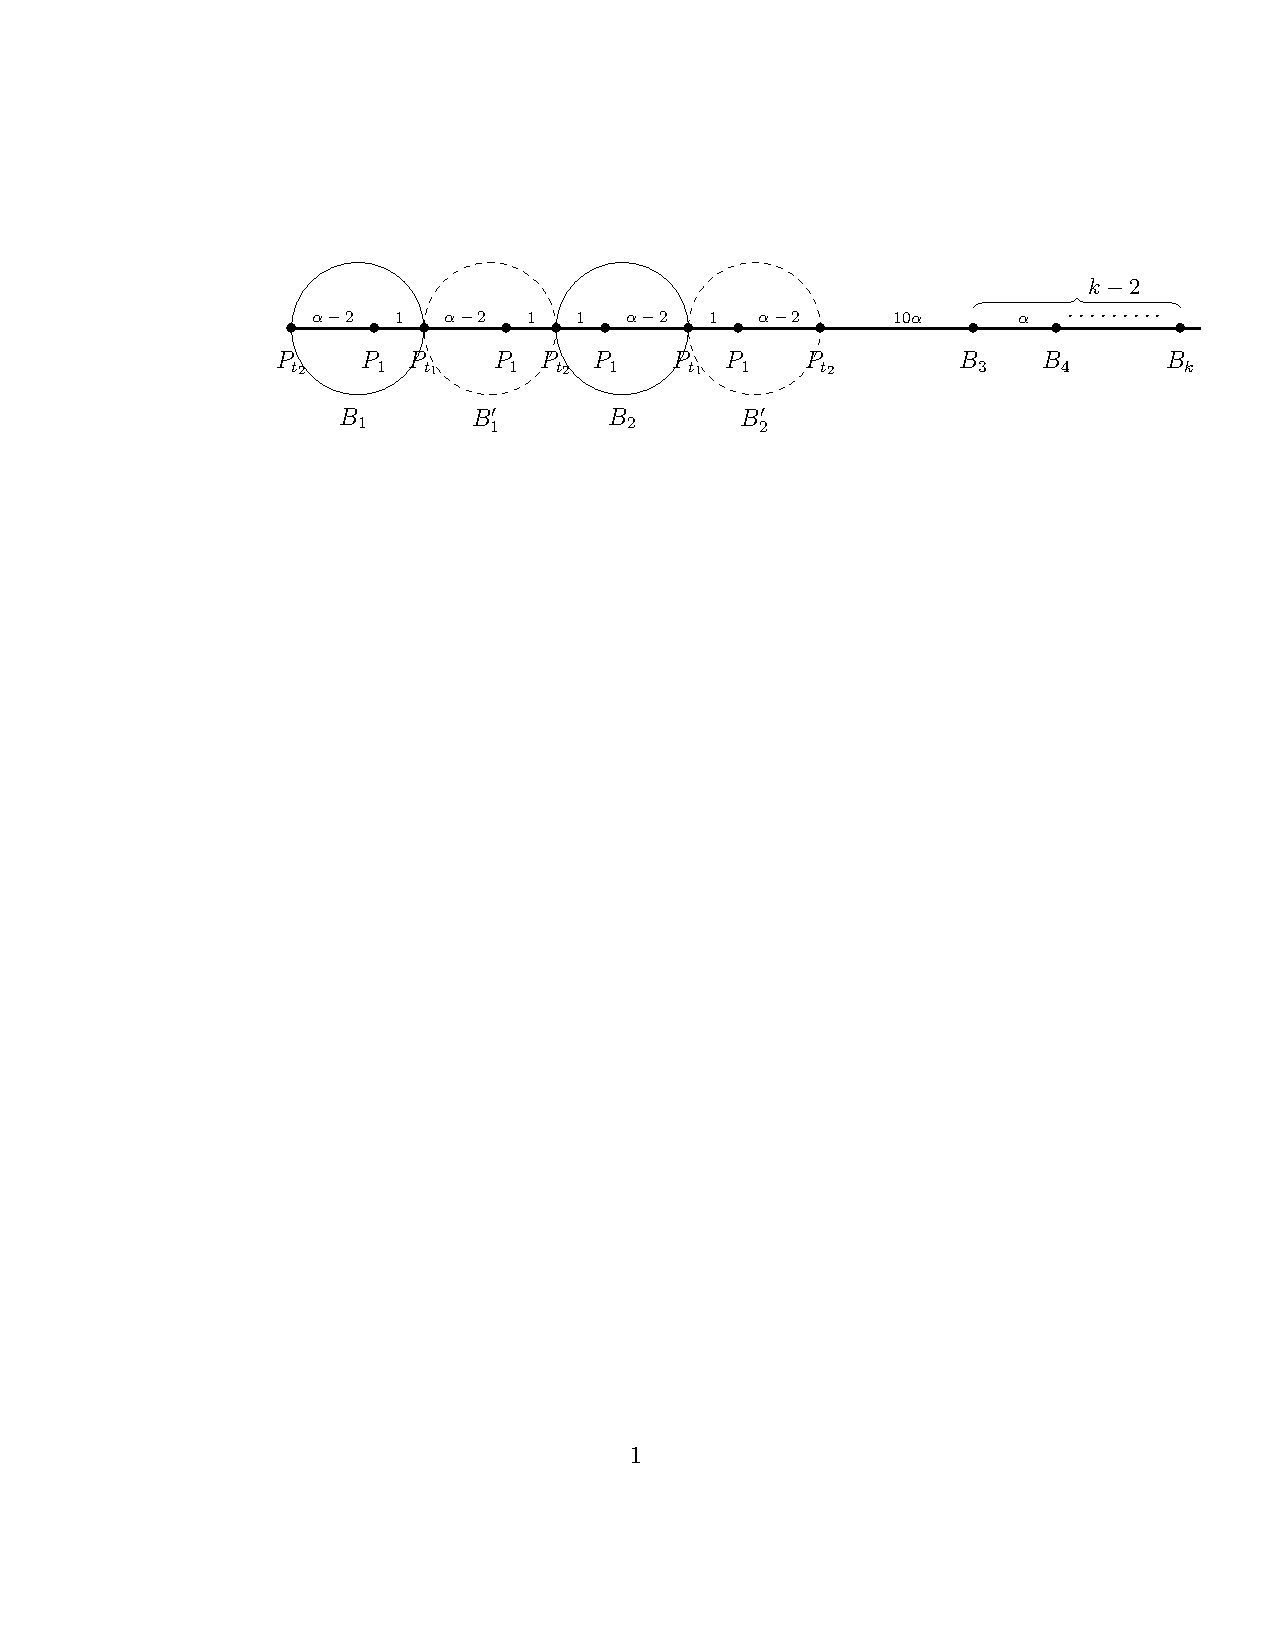
\includegraphics[trim={35mm 235mm 20mm 20mm},clip,width=\textwidth]{figures/lbdFig2}
\end{center}
\vspace{-1cm}
\caption{$\mc X \subseteq \mathbb{R}$ such that no tree can capture all the $(\alpha, \eta)$-proximal clusterings.}
\label{fig:noalgalphacp}
\end{figure}

Assume that there exists a tree $T$ and prunings $P$ and $P'$ such that $P$ respects $\mc C_{\mc S}$ and $P'$ respects $\mc C_{\mc S'}$. Hence,  $\exists N_1$ such that $B_1 \subseteq N_1$ and $N_1 \cap B_2 = \phi$ and $\exists N_2$ such that $B_2 \subseteq N_2$ and $N_2 \cap B_1 = \phi$. Similarly, $\exists N_1'$ such that $B_1' \subseteq N_1'$ and $N_1' \cap B_2' = \phi$. Now, $B_1'$ contains points from both $B_1$ and $B_2$. Hence, both $N_1 \subseteq N_1'$ and $N_2 \subseteq N_1'$. Thus, $P_{t'}(3\alpha-3)\in B_2'\cap B_2 \subseteq B_2' \cap N_2 \subseteq B_2' \cap N_1'$. This is a contradiction.
\qed\\

\noindent\textbf{Proof of Thm. \ref{thm:nolistalphacp}}
The clustering instance $\mc X$ is a simple extension of our tree example (Fig. \ref{fig:noalgalphacp}). In the tree example $ 4$ balls were placed side-by-side one another. Let  $G_1 = \{B_1, B_1', B_2, B_2'\}$ be the balls as in Fig. \ref{fig:noalgalphacp}. Now, construct $G_2 = \{B_3, B_3', B_4, B_4'\}$ exactly identical to $G_1$ but far. In this way, we cosntruct $k/2$ copies of $G_1$. Now, it easy to see that any list $\mc L$ should have size at least $2^{k/2}$.\qed\\


\noindent\textbf{Proof of Thm. \ref{thm:nosparsealg}}
Let $\mc X \subseteq \mathbb{R}$ be as shown in Fig. \ref{fig:nosparsealg}. Let $t' = \frac{t}{2}-1$ and let $B_1, B_2, B_3, B_1'$, $B_2', B_3', B_1'', B_2''$ and $B_3''$ be as shown in Fig. \ref{fig:nosparsealg}. For $\alpha \le 2\sqrt{2}+3$, clusterings $\mc C_{\mc S} = \{B_1, B_2, B_3, \ldots, B_k\}$, $\mc C_{\mc S'} = \{\ B_1', B_2', B_3, \ldots, B_k\}$ and $\mc C_{\mc S}'' = \{\ B_1'', B_2'', B_3, \ldots, B_k\}$ satisfy $(\alpha, 1)$-center proximity. Also, $m(\mc C_{\mc S}) = m(\mc C_{\mc S}') =$ $m(\mc C_{\mc S}'') = t$. Arguing similarly as in Thm. \ref{thm:noalgalphacp} completes the proof. \qed\\
\begin{figure}[!t]
\vspace{-5mm}
\begin{center}
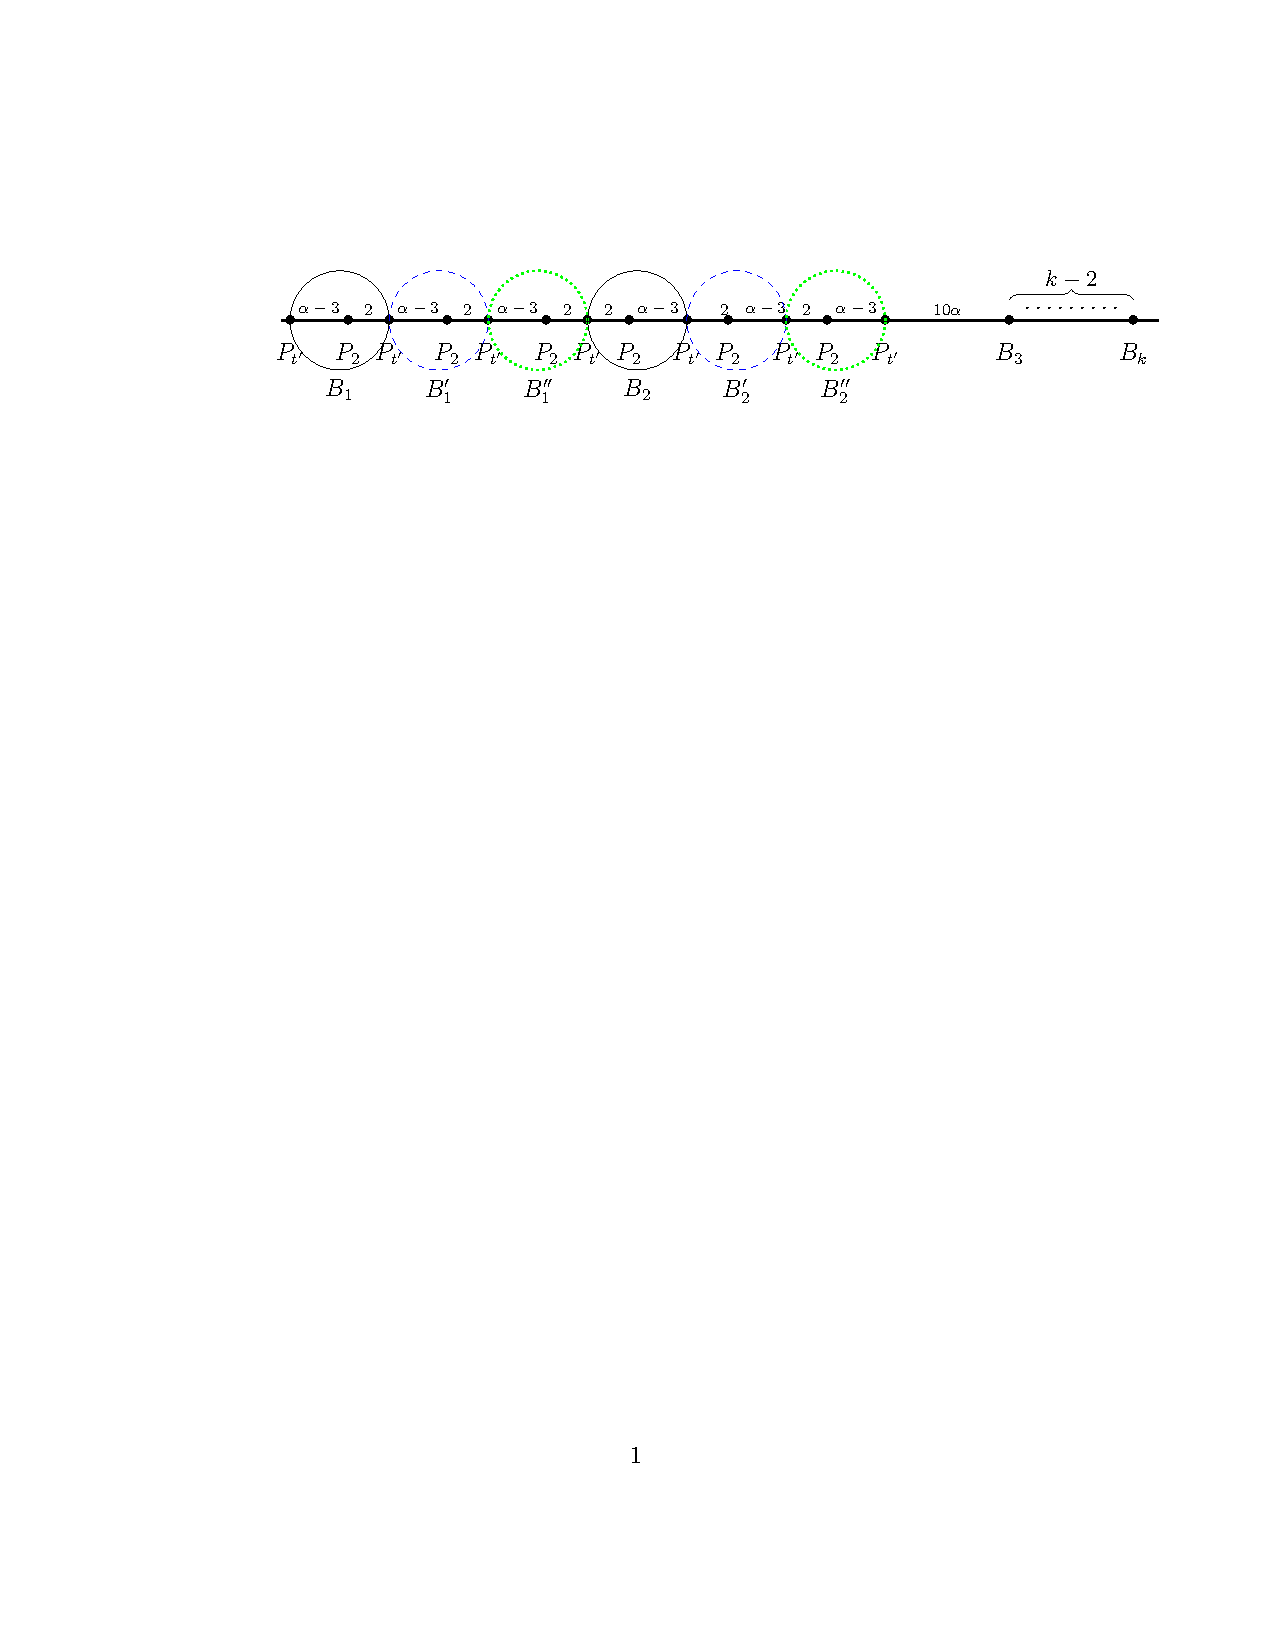
\includegraphics[trim={40mm 210mm 20mm 40mm},clip,width=\textwidth]{figures/lbdFig3}
\end{center}
\vspace{-4mm}
\caption{$\mc X \subseteq \mathbb{R}$ such that no algorithm can capture all the $\alpha$-proximal clusterings. } 
\label{fig:nosparsealg}
\end{figure}

\noindent\textbf{Proofs of Thms. \ref{thm:nosparselistalphacp}, \ref{thm:nosparselistlambdacs} and \ref{thm:nolistlambdacs}} have the exact same ideas as the proof of Thm. \ref{thm:nolistalphacp}. To prove the lower bound in the list model, instance constructed in Thm. \ref{thm:nolistalphacp} is a `simple' extension of the instance constructed in the proof of tree lower bound (Thm. \ref{thm:noalgalphacp}). The instances for the proof of Thms. \ref{thm:nosparselistalphacp}, \ref{thm:nosparselistlambdacs} and \ref{thm:nolistlambdacs} are similarly constructed as extensions of their respective tree lower bound instances (Thms. \ref{thm:nosparsealg}, \ref{thm:nosparselambdaalg} and \ref{thm:noalglambdacs} respectively).\\

\noindent\textbf{Proof of Thm. \ref{thm:lambdaNoNoisePositive}}
We say that a clustering $\mc C_{\mc X}$ has strong stability \cite{balcan2008discriminative} when for all $C_i, C_j \in \mc C_{\mc X}$ and for all $A \subset C_i$, $A' \subseteq C_j$, we have that $d_{min}(A, C_i\setminus A) < d_{min}(A, A')$ where $d_{min}(A, B) = \min \{d(a, b): a \in A$ and $b \in B\}$.  .  We will now show that $\mc C_{\mc X}^*$ has strong stability which will complete the proof (Theorem. 8 in \cite{balcan2008discriminative}). Let $A \subset C_i^*$ and $B \subseteq C_j^*$. 

Let $p \in A$ and $q \in C_i^* \setminus A$ be points which achieve the minimum distance between $A$ and $C_i^*\setminus A$. If $c_i \in A$ then $d(p, q) \le d(c_i, q) \le r$. If $c_i \in C_i^* \setminus A$ then $d(p, q) \le d(p, c_i) \le r$. Hence, $d_{min} (A, C_i^*\setminus A) \le r$. Let $p \in A$ and $s \in B$ be points which achieve the minimum distance between $A$ and $B$. Using triangle inequality, we get that $d_{min}(A, B) = d(p, s) \ge d(c_i, c_j) - d(p, c_i) - d(s, c_j) > 3r - r - r = r$.\qed

\noindent\textbf{Proof of Thms. \ref{thm:nosparselambdaalg} and \ref{thm:noalglambdacs}}
The clustering instance $\mc X$ is the same as the corresponding $\alpha$-center proximity instances. The only difference is that the distances between the adjacent points are the same (equal to the given parameter $r$ instead of $\alpha-2$ or $1$ or $\alpha-1$). The proofs are also identical to the proofs of Thm. \ref{thm:nosparsealg} and \ref{thm:noalgalphacp} respectively. \qed

\noindent\textbf{Proof of Thm. \ref{thm:lambdacsnoise}}
Fix $\mc S \subseteq \mc X$. Denote by $r_i := r(S_i^*)$. Let $\mc C_{\mc X} = \{C_1, \ldots, C_k\}$ be the clustering outputed by the algorithm. Let $\mc L = \{B_1, \ldots, B_l\}$ be the list of balls as outputed by Phase 1 of Alg. \ref{alg:lambdacs}. Let $G$ be the graph as constructed in Phase 2 of the algorithm. Observe that $B = B(s_i, r_i) = S_i^* \in \mc L$. WLOG, denote this ball by $B^{(i)}$ and the corresponding vertex in the graph $G$ by $v^{(i)}$. We will prove the theorem by proving two key facts.  

\begin{enumerate}[nolistsep,noitemsep,label=\textbf{F.\arabic*}]
\renewcommand\labelitemi{$\diamond$}
\item \label{fact:lambda1} If $B_{i1}$ and $B_{i2}$ intersect $S_i^*$ then the vertices $v_{i1}$ and $v_{i2}$ are connected.
\item \label{fact:lambda2} If $B_{i1}$ intersects $S_i^*$ and $B_{j1}$ intersects $S_j^*$ then $v_{i1}$ and $v_{j1}$ are disconnected in $G$.	
\end{enumerate}

\begin{smallLemma}
\label{claim:lambda1}
Let $\mc L, G, B^{(i)}$ and $v^{(i)}$ be as defined above. Let balls $B_{i1}, B_{i2} \in \mc L$ be such that $B_{i1} \cap S_i^* \neq \phi$ and $B_{i2} \cap S_i^* \neq \phi$. Then there exists a path between $v_{i1}$ and $v_{i2}$.
\end{smallLemma}
\vspace{-0.1in} Assume that $v_{i1}$ and $v^{(i)}$ are not connected by an edge. Hence, $|B_{i1} \setminus B^{(i)}| \ge t/2$. Since $\lambda > 4$, for all $j \neq i$, $B_{i1} \cap S_j^* = \phi$. Thus, $B_{i1} \setminus B^{(i)} \subseteq \mc X \setminus \mc S$. which contradicts $|B_{i1} \cap \{\mc X \setminus \mc S\}| < t/2$.\qed

\begin{smallLemma}
Let the framework be as in Claim \ref{claim:lambda1}. Let $B_{i1} \in \mc L$ be such that $B_{i1} \cap S_i^* \neq \phi$ and $B_{j1}$ be such that $B_{j1} \cap S_j^* \neq \phi$. Then $v_{i1}$ and $v_{j1}$ are disconnected in $G$.
\end{smallLemma}
\vspace{-0.1in} Assume that $v_{i1}$ and $v_{j1}$ are connected. Hence, there exists vertices $v_{i}$ and $v_{n}$ such that $v_i$ and $v_n$ are connected by an edge in $G$ and $B_i \cap S_i^* \neq \phi$ and $B_n \cap S_n^* \neq \phi$ for some $n \neq i$. $|B_i \cap B_n| \ge t/2$. Now, $\lambda \ge 4$, thus $B_i \cap \{\mc S \setminus S_i^*\} = \phi$ and $B_n \cap \{\mc S\setminus S_n^*\} = \phi$. Thus, $B_i \cap B_n \subseteq \mc X \setminus \mc S$ which contradicts the sparseness assumption.
\qed

\label{appendix:sectiontr}
\begin{theorem}[Vapnik and Chervonenkis \cite{vapnik2015uniform}]\label{theorem:vceapprox}
Let $X$ be a domain set and $D$ a probability distribution over $X$. Let $H$ be a class of subsets of $X$ of finite VC-dimension $d$. Let $\epsilon, \delta \in (0,1)$. Let $S \subseteq X$ be picked i.i.d according to $D$ of size $m$. If $m > \frac{c}{\epsilon^2}(d\log \frac{d}{\epsilon}+\log\frac{1}{\delta})$, then  with probability $1-\delta$ over the choice of $S$, we have that $\forall h \in H$
$$\bigg|\frac{|h\cap S|}{|S|} - P(h)\bigg| < \epsilon$$
\end{theorem}


\end{document}
